\section{1174006 - Kadek Diva Krishna Murti}

\subsection{Teori}
\subsubsection{Definisi Kecerdasan Buatan}
\hfill\break
Kecerdasan buatan atau artificial intelligence (AI) menurut beberapa pakar adalah sebagai berikut:
\begin{enumerate}
	\item Schalkoff (1990): AI adalah bidang studi yang mencoba meniru dan menerangkan perilaku cerdas yang dilakukan oleh manusia dalam bentuk proses komputasi.
	\item Rich dan Knight (1991): AI adalah studi tentang cara membuat komputer melakukan sesuatu yang sampai saat ini orang dapat melakukannya lebih baik.
	\item Luger dan Stubblefield (1993): AI adalah cabang ilmu komputer yang berhubungan dengan otomasi perilaku yang cerdas.
	\item Keen dan Haag (1996): AI adalah cabang ilmu komputer yang berkaitan dengan pemodelan, penangkapan, dan penyimpanan kecerdasan manusia ke dalam sebuah sistem teknologi informasi sehingga sistem tersebut nantinya dapat memfasilitasi dalam melakukan pengambilan keputusan yang biasanya dilakukan oleh manusia.
\end{enumerate}
\noindent
Jadi dapat disimpulkan kecerdasan buatan atau artificial intelligence (AI) merupakan salah satu bagian ilmu komputer yang membuat mesin (komputer) dapat melakukan pekerjaan seperti dan sebaik yang dilakukan oleh manusia. Seperti yang kita tahu pada awal diciptakannya, komputer hanya difungsikan sebagai alat hitung saja. Namun seiring dengan perkembangan jaman, maka peran komputer semakin mendominasi kehidupan umat manusia. Komputer tidak lagi sekedar digunakan sebagai alat hitungn namun diharapkan untuk dapat diberdayakan untuk mengerjakan segala sesuatu yang bisa dikerjakan oleh manusia.

\subsubsection{Sejarah dan Perkembangan Kercerdasan Buatan}
\hfill\break
Istilah AI pertama kali dikemukakan pada tahun 1956 dikonferensi Darthmouth. Sejak saat itu AI terus dikembangkan sebab berbagai penelitian mengenai teori-teori dan prinsip-prinsipnya juga terus berkembang. Meskipun istilah AI baru muncul tahun 1956, tetapi teori-teori mengarah ke AI sudah muncul sejak tahun 1941. Berikut ini tahapan-tahapan sejarah perkembangan AI:
\begin{enumerate}
	\item Era Komputer Elektronik (1941)
	\hfill\break
	Pada tahun 1941 telah ditemukan alat penyimpanan dan pemrosesan informasi. Penemuan tersebut dinamakan komputer elektronik yang dikembangkan di USA dan Jerman. Komputer pertama ini memerlukan ruangan yang luas dan ruang AC yang terpisah. Saat itu komputer meibatkan konfigurasi ribuan kabel untuk menjalankan suatu program. Hal ini sangat merepotkan bagi para programmer. Pada tahun 1949, berhasil dibuat komputer yang mampu menyimpan program sehingga membuat pekerjaan untuk memasukkan program menjadi lebih mudah. Penemuan ini menjadi dasar pengembangan program yang mengarah ke AI.

	\item Masa Persiapan AI (1943–1956)
	\hfill\break
	Pada tahun 1943, Warren McCulloch dan Walter Pitts mengemukakan tiga hal: pengetahuan fisiologi dasar dan fungsi sel syaraf dalam otak, analisis formal tentang logika proporsi (propositional logic), dan teori komputasi turing. Mereka berhasil membuat suatu model syaraf tiruan (artificial neuron) di mana setiap neuron digambarkan sebagai on dan off. Mereka menunjukkan bahwa setiap fungsi dapat dihitung dengan suatu jaringan sel syaraf dan bahwa semua hubungan logis dapat diimplementasikan dengan struktur jaringan yang sederhana.
	\noindent
	Pada tahun 1950, Norbert Wiener mebuat penelitian mengenai prinsip-prinsip teori feedback. Contoh yang terkenal adalah thermostat. Penemuan ini juga merupakan awal perkembangan AI. Pada tahun 1956, John McCarthy (yang setelah lulus dari Princeton kemudian melanjutkan ke Dartmouth College) meyakinkan Minsky, Claude Shannon dan Nathaniel Rochester untuk membantunya melakukan penelitian dalam bidang Automata, jaringan sel syaraf dan pembelajaran intelejensia. Mereka mengerjakan proyek ini selama dua bulan di Dartmouth. Hasilnya adalah program yang mampu ber-pikir non-numerik dan menyelesaikan masalah pemikiran, yang dinamakan Principia Mathematica. Hal ini menjadikan McCarthy disebut sebagai Father of AI (Bapak AI).

	\item Awal Perkembangan AI (1952–1969)
	\hfill\break
	Pada tahun-tahun pertama pengembangannya, AI mengalami banyak kesuksesan. Diawali dengan kesuksesan Newell dan Simon dengan sebuah program yang disebut General Problem Solver. Program ini dirancang untuk memulai penyelesaian masalah secara manusiawi. Pada tahun 1958, McCarthy di MTT Lab Memo No. 1 mendefinisikan bahasa pemrograman tingkat tinggi yaitu LISP, yang sekarang mendominasi pembuatan program-program AI. Kemudian, McCarthy membuat program yang dinamakan Programs With Common Sense. Di dalam program tersebut, dibuat rancangan untuk menggunakan pengetahuan dalam mencari solusi. Pada tahun 1959, Nathaniel Rochester dari IBM dan mahasiswa-mahasiswanya mengeluarkan program AI Geometry Theorm Prover. Program ini dapat membuktikan suatu teorema menggunakan axioma-axioma yang ada. Pada tahun 1963, program yang dibuat James Slagle mampu menyelesaikan masalah integral tertutup untuk mata kuliah kalkulus. Pada tahun 1968, program analogi buatan Tom Evan menyelesaikan masalah analogi geometris yang ada pada tes IQ.

	\item Perkembangan AI Melambat (1966–1974)
	\hfill\break
	Prediksi Herbert Simon pada tahun 1957 yang menyatakan bahwa AI akan menjadi ilmu pengetahuan yang akan berkembang dengan pesat ternyata meleset. Pada 10 tahun kemudian, perkembangan AI melambat. Hal ini disebabkan adanya 3 kesulitan utama yang dihadapi AI, yaitu:
	\begin{enumerate}
		\item Masalah pertama: program-program AI yang bermunculan hanya mangandung sedikit atau bahkan tidak mengandung sama sekali pengetahuan (knowledge) pada subjeknya. Program-program AI berhasil hanya karena manipulasi sintetis yang sederhana. Sebagai contoh adalah Weizenbaum’s ELIZA program (1965) yang dapat melakukan percakapan serius pada berbagai topik, sebenarnya hanyalah peminjaman dan manipulasi kalimat-kalimat yang diketikkan oleh manusia.
		\item Masalah kedua: banyak masalah yang harus diselesaikan oleh AI. Karena terlalu banyaknya masalah yang berkaitan, maka tidak jarang banyak terjadi kegagalan pada pembuatan program AI.
		\item Masalah ketiga: ada beberapa batasan pada struktur dasar yang digunakan untuk menghasilkan perilaku intelejensia. Sebagai contoh adalah pada tahun 1969 buku Minsky dan Papert Perceptrons membuktikan bahwa program-program perceptrons dapat mempelajari segala sesuatu, tetapi program-program tersebut hanya mempresentasikan sejumlah kecil saja. Sebagai contoh dua masukan perceptrons yang berbeda tidak dapat dilatihkan untuk mengenali kedua masukan yang berbeda tersebut.
	\end{enumerate}

	\item Sistem Berbasis Pengetahuan (1969–1979)
	\hfill\break
	Pengetahuan adalah kekuatan pendukung AI. Hal ini dibuktiikan dengan program yang dibuat oleh Ed Feigenbaum,Bruce Buchanan dan Joshua Lederberg yang membuat program untuk memecahkan masalah struktur molekul dari informasi yang didapatkan dari spectometer massa. Program ini dinamakan Dendral programs yang berfokus pada segi pengetahuan kimia. Dari segi diagnosis media juga sudah ada yang menemukannya, yaitu Saul Amarel dalam proyek computer in biomedicine. Proyek ini diawali dari keinginan untuk mendapatkan diagnosa penyakit berdasarkan pengetahuan yang ada pada mekanisme penyebab proses penyakit.

	\item AI Menjadi Sebuah Industri (1980–1988)
	\hfill\break
	Industrialisasi AI diawali dengan ditemukannya expert system (sistem pakar) yang dinamakan R1 yang mampu mengkonfigurasi sistem-sistem komputer baru. Program tersebut mulai dioperasikan di Digital Equipment Corporation(DEC), McDermott, pada tahun 1982. Pada tahun 1986, program ini telah berhasil menghemat US\$40 juta per tahun. Pada tahun 1988, kelompok AI di DEC menjalankan 40 sistem pakar. Hampir semua perusahaan besar di USA mempunyai divisi AI sendiri yang menggunakan ataupun mempelajari sistem pakar. Booming industri AI ini juga melibatkan perusahaan-perusahaan besar seperti Carnegie Group, Inference, Intellicorp, dan Technoledge yang menawarkan software tools untuk membangun sistem pakar. Perusahaan hardware seperti LISP dan Machines Inc., Texas Instruments, Symbolics, dan Xerox juga turut berperan dalam membangun workstation yang dioptimasi untuk pembangunan program LISP. Sehingga, perusahaan yang sejak tahun 1982 hanya menghasilkan beberapa juta US dolar per tahun meningkat menjadi 2 milyar US dolar per tahun pada tahun 1988.

	\item Kembalinya Jaringan Syaraf Tiruan (1986–Sekarang)
	\hfill\break
	Meskipun bidang ilmu komputer menolak jaringan syaraf tiruan setelah diterbitkannya buku "perceptrons" karangan Minsky dan Papert, tetapi para ilmuan masih mempelajari bidang ilmu tersebut dari sudut pandang yang lain yaitu fisika. Para ahli seperti Hopfield (1982) menggunakan teknik-teknik mekanika statistika untuk menganalisa sifat-sifat penyimpanan dan optimasi pada jaringan syaraf. Para ahli psikollogi, David Rumelhart dan Geoff Hinton, melanjutkan penelitian mengenai model syaraf pada memori. Pada tahun 1985-an sedikitnya empat kelompok riset menemukan kembali algoritma belajar propagasi balik (Back-Propagation Learning). Algoritma ini berhasil diimplementasikan kedalam bidang ilmu komputer dan psikologi.

\end{enumerate}

\subsubsection{Supervised Learning}
\hfill\break
Supervised Learning adalah pembelajaran yang memiliki label di tiap datanya. Label maksudnya adalah tag dari data yang ditambahkan dalam machine learning model. Contohnya gambar kucing di tag "kucing" di tiap masing masing image kucing dan gambar anjing di tag "anjing" di tiap masing gambar anjing. Machine learning kategori dapat berupa clasification ("anjing", "kucing", "beruang", dsb) dan regression ( berat badan, tinggi badan dsb). Supervised learning banyak digunakan dalam memprediksi pola dimana pola tersebut sudah ada contoh data yang lengkap, jadi pola yang terbentuk adalah hasil pembelajaran data lengkap tersebut. Tentunya jika kita memasukan data baru, setelah kita melakukan ETL (Extract Transform Load) maka kita mendapat info feature feature dari sample baru tersebut. Kemudian dari feature feature tersebut di compare dengan pattern clasification dari model yang didapat dari labeled data. Setiap label akan dicompare sampai selesai, dan yang memiliki percentage lebih banyak akan diambil sebagai prediksi akhir.

\begin{figure}[H]
	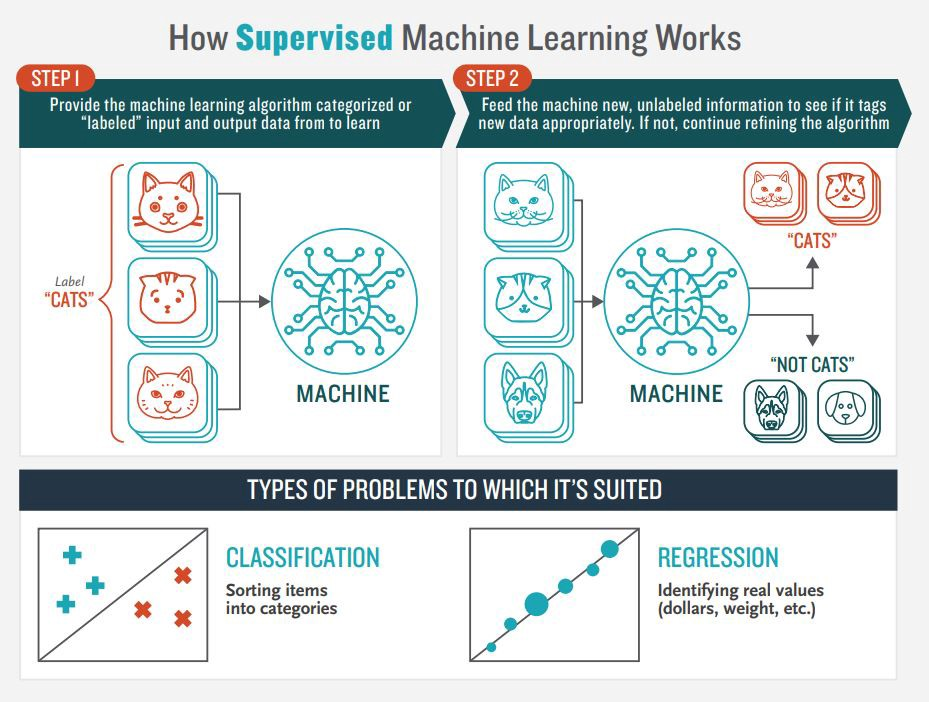
\includegraphics[width=1\textwidth]{figures/1174006/chapter1/supervisedlearning.jpeg}
	\centering
	\caption{Supervised Learning.}
\end{figure}
\noindent
Contoh algoritma yang digunakan pada supervised learning meliputi :
\begin{enumerate}
	\item Clasification (Categorical) and Regression (Numerical)
    \item Logistic Regression
    \item Model Ensemble
	\item Time series
\end{enumerate}

\subsubsection{Klasifikasi}
\hfill\break
Classification adalah tindakan untuk memberikan kelompok pada setiap keadaan. Setiap keadaan berisi sekelompok atribut, salah satunya adalah class attribute. Metode ini butuh untuk menemukan sebuah model yang dapat menjelaskan class attribute itu sebagai fungsi dari input attribute.
\begin{figure}[H]
	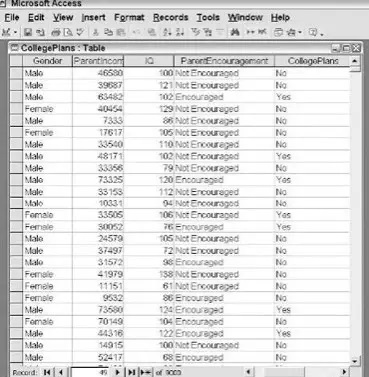
\includegraphics[width=1\textwidth]{figures/1174006/chapter1/clasification.jpg}
	\centering
	\caption{Clasification.}
\end{figure}
\noindent
Class adalah attribute CollegePlans yang berisi dua pernyataan, Yes dan No, perhatikan ini.
\noindent
Sebuah Classification Model akan menggunakan atribut lain dari kasus tersebut (input attribut; yaitu kolom IQ, Gender, ParentIncome, dan ParentEncouragement) untuk dapat menentukan pola (pattern) class (Output Attribute; yaitu Kolom CollegePlans yang berisi Yes atau No).
\noindent
Algoritma Data Mining yang membutuhkan variabel target untuk belajar (sampai mendapatkan rule / pola yang berlaku pada data tersebut) kita standarkan dengan sebuthan dengan Supervised Algorithm.
\noindent
Nah, yang termasuk kepada Classification Algorithm adalah Decision Trees, Neural Network dan Naives Bayes.
\subsubsection{Regresi}
\hfill\break
Metode Regression mirip dengan metode Classification, yang membedakannya adalah metode regression tidak bisa mencari pola yang dijabarkan sebagai class (kelas).
\noindent
Metoda regression bertujuan untuk mecari pola dan menentukan sebuah nilai numerik.
\noindent
Sebuah Teknik Linear Line-fitting sederhana adalah sebuah contoh dari Regression, dimana hasilnya adalah sebuah fungsi untuk menentukan hasil yang berdasarkan nilai dari input.
\noindent
Bentuk yang lebih canggih dari regression sudah mendukung input berupa kategori, jadi tidak hanya input berupa numerik. Teknik paling popular yang digunakan untuk regression adalah linear regression dan logistic regression. Teknik lain yang didukung oleh SQL Server Data mining adalah Regression Trees (bagian dari dari algoritma Microsoft Decission Trees) dan Neural Network.
\noindent
Regression digunakan untuk memecahkan banyak problem bisnis – contohnya untuk memperkirakan metode distribusi, kapasitas distribusi, musim dan untuk memperkirakan kecepatan angin berdasarkan temperatur, tekanan udara, dan kelembaban.
\subsubsection{Unsupervised Learning}
\hfill\break
Unsupervised learning memiliki keunggulan dari supervised learning. Jika supervised learning memiliki label sebagai dasar prediksi baik serta membuat clasification dan regression algorithm memungkinkan. Tetapi dalam realitanya, data real itu banyak yang tidak memiliki label. Label kebanyakan jika data sudah masuk ke ERP apapun bentuk ERPnya dan bagaimana kalo datanya berupa natural input seperti suara, gambar, dan video. Unsupervised learning tidak menggunakan label dalam memprediksi target feautures / variable. Melainkan menggunakan ke samaan dari attribut attribut yang dimiliki. Jika attribut dan sifat-sifat dari data data feature yang diekstrak memiliki kemirip miripan, maka akan dikelompok kelompokan (clustering). Sehingga hal ini akan menimbulkan kelompok kelompok (cluster). Jumlah cluster bisa unlimited. Dari kelompok kelompok itu model melabelkan, dan jika data baru mau di prediksi, maka akan dicocok kan dengan kelompok yang mirip mirip featurenya.
\begin{figure}[H]
	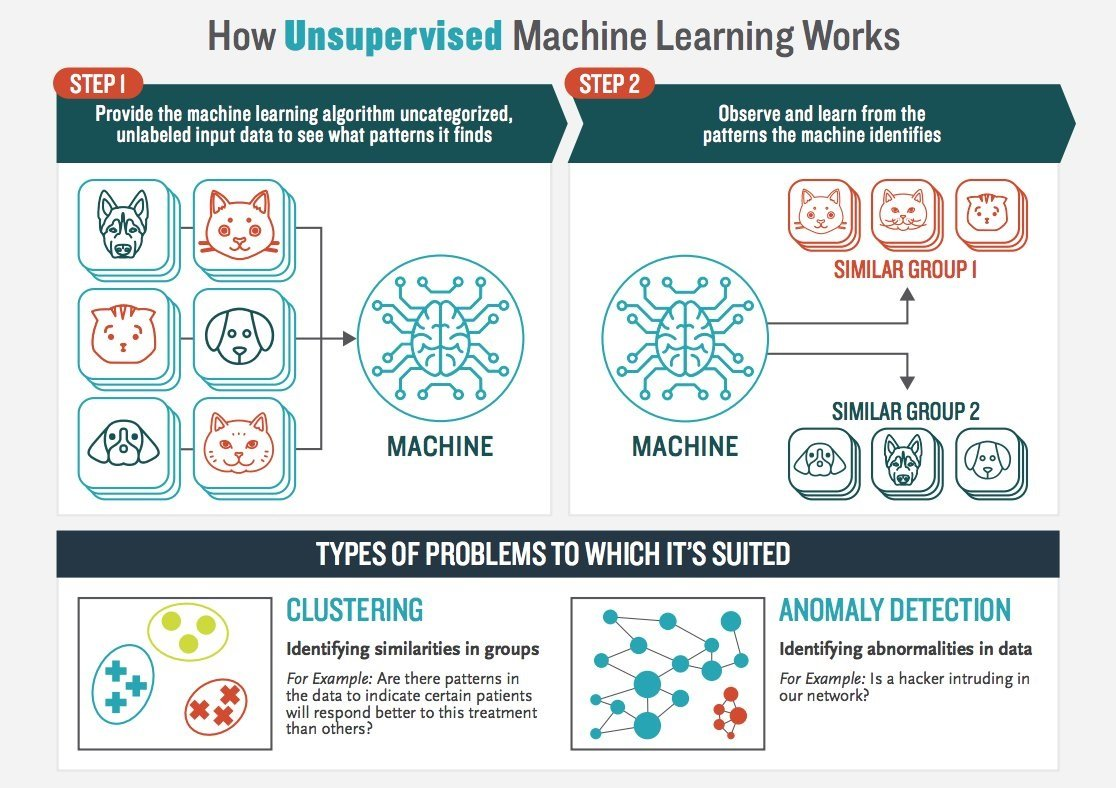
\includegraphics[width=1\textwidth]{figures/1174006/chapter1/unsupervisedlearning.jpg}
	\centering
	\caption{Unsupervised Learning.}
\end{figure}
\noindent
Tetapi unsupervise learning tidak memiliki outcome yang spesifik layaknya di supervise learning, hal ini dikarenakan tidak adanya ground truth / label dasar. Walaupun begitu, unsupervised learning masih dapat memprediksi dari ketidakadaan label dari kemiripan attribute yang dimilik data.
\noindent
Algoritma yang digunakan di unsupervised learning :
\begin{enumerate}
	\item Clustering
    \item Anomaly Detection
    \item Training Model
    \item Association Discovery
\end{enumerate}
\subsubsection{Data Set}
\hfill\break
Dataset adalah objek yang merepresentasikan data dan relasinya di memory. Strukturnya mirip dengan data di database. Dataset berisi koleksi dari datatable dan data relation.
\subsubsection{Training Set}
\hfill\break
Training set adalah bagian dataset yang kita latih untuk membuat prediksi atau menjalankan fungsi dari sebuah algoritma ML lainnya sesuai tujuannya masing-masing. Kita memberikan petunjuk melalui algoritma agar mesin yang kita latih bisa mencari korelasinya sendiri. 
\subsubsection{Testing Set}
\hfill\break
Test set adalah bagian dataset yang kita tes untuk melihat keakuratannya, atau dengan kata lain melihat performanya.
\subsection{Praktek}
\begin{enumerate}
	\item Instalasi  library  scikit  dari  anaconda,  mencoba  kompilasi  dan  uji  coba  ambil contoh kode dan lihat variabel explorer.
	
	\textbf{Instalasi Library Scikit-Learn dengan Anaconda}
	\begin{enumerate}
		\item Pertama pastikan anda telah menginstall Anaconda. Jika sudah menginstall Anaconda, jalankan Anaconda Navigator.
		\begin{figure}[H]
			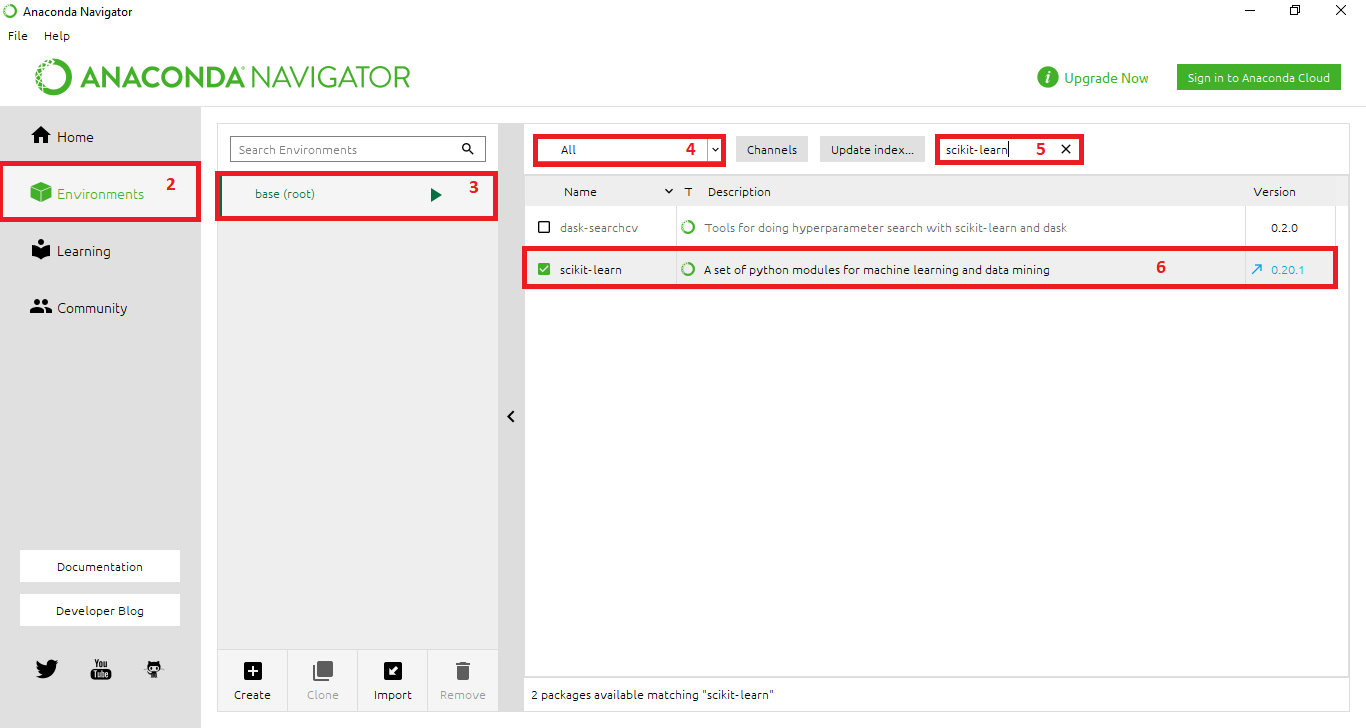
\includegraphics[width=1\textwidth]{figures/1174006/chapter1/praktek/install.png}
			\centering
			\caption{Instalasi Library Scikit-Learn.}
		\end{figure}
		\item Selanjutnya klik menu Environment.
		\item Kemudian klik environment base(root). Disini kita akan melakukan instalasi library scikit- learn di environment base(root).
		\item Lalu pilih All. Untuk menampilkan list library yang ada.
		\item Setelah itu cari scikit-learn di kolom pencarian.
		\item Selanjutnya centang library scikit-learn, lalu klik tombol Apply.
	\end{enumerate}

	\textbf{Mencoba Menggunakan Library scikit-Learn}
	\begin{enumerate}
		\item Pertama jalankan aplikasi Spyder.
		\item Kemudian buat file baru, lalu tambahkan kode berikut.
		\lstinputlisting[language=Python]{src/1174006/chapter1/contoh.py}
		\item Simpan dan jalankan.
		\item Hasil dari variabel explorernya sebagai berikut.
		\begin{figure}[H]
			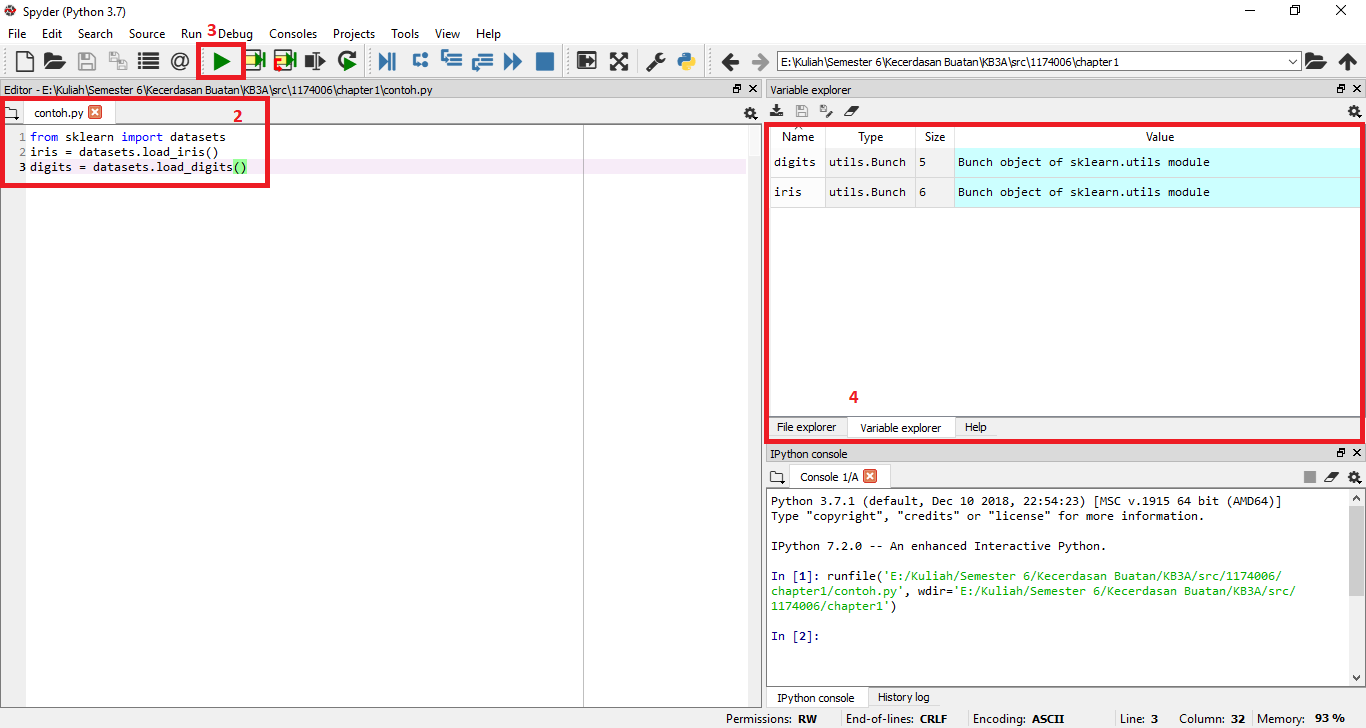
\includegraphics[width=1\textwidth]{figures/1174006/chapter1/praktek/variabel.png}
			\centering
			\caption{Variabel Explorer Library Scikit-Learn.}
		\end{figure}
	\end{enumerate}
	
	\item Mencoba Loading an example dataset, menjelaskan maksud dari tulisan terse-but dan mengartikan per baris.
	\lstinputlisting[language=Python]{src/1174006/chapter1/coba1.py}
	
	Hasilnya akan seperti ini.
	\begin{figure}[H]
		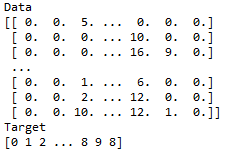
\includegraphics[width=5cm]{figures/1174006/chapter1/praktek/coba1.png}
		\centering
		\caption{Hasil Loading an Example Dataset.}
	\end{figure}

	\item Mencoba  Learning  and  predicting,  menjelaskan  maksud  dari  tulisan  tersebut dan mengartikan per baris.
	\lstinputlisting[language=Python]{src/1174006/chapter1/coba2.py}
	
	Hasilnya akan seperti ini.
	\begin{figure}[H]
		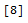
\includegraphics[width=1cm]{figures/1174006/chapter1/praktek/coba2.png}
		\centering
		\caption{Hasil Learning and Predicting.}
	\end{figure}

	\item Mencoba Model persistence, menjelaskan maksud dari tulisan tersebut dan mengartikan per baris.
	\lstinputlisting[language=Python]{src/1174006/chapter1/coba3.py}
	
	Hasilnya akan seperti ini.
	\begin{figure}[H]
		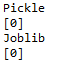
\includegraphics[width=2cm]{figures/1174006/chapter1/praktek/coba3.png}
		\centering
		\caption{Hasil Model Persistence.}
	\end{figure}

	\item Mencoba Conventions, menjelaskan maksud dari tulisan tersebut dan mengartikan per baris.
	\lstinputlisting[language=Python]{src/1174006/chapter1/coba4.py}
	
	Hasilnya akan seperti ini.
	\begin{figure}[H]
		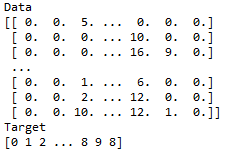
\includegraphics[width=5cm]{figures/1174006/chapter1/praktek/coba1.png}
		\centering
		\caption{Hasil Conventions.}
	\end{figure}

\end{enumerate}

\subsection{Penanganan Error}
\begin{enumerate}
	\item Skrinsut error.
	\begin{itemize}
		\item Name Error
		\hfill\break
		\begin{figure}[H]
			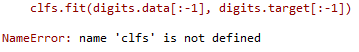
\includegraphics[width=1\textwidth]{figures/1174006/chapter1/error/err3.png}
			\centering
			\caption{Name Error.}
		\end{figure}
		\item Import Error
		\hfill\break
		\begin{figure}[H]
			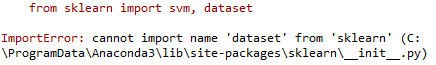
\includegraphics[width=1\textwidth]{figures/1174006/chapter1/error/err1.png}
			\centering
			\caption{Import Error.}
		\end{figure}
		\item Value Error
		\hfill\break
		\begin{figure}[H]
			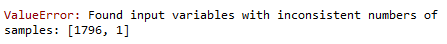
\includegraphics[width=1\textwidth]{figures/1174006/chapter1/error/err2.png}
			\centering
			\caption{Value Error.}
		\end{figure}
		\item Syntax Error
		\hfill\break
		\begin{figure}[H]
			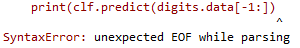
\includegraphics[width=1\textwidth]{figures/1174006/chapter1/error/err4.png}
			\centering
			\caption{Syntax Error.}
		\end{figure}
	\end{itemize}
	\item Tuliskan kode eror dan jenis errornya.
	\begin{itemize}
		\item Name Error
		\hfill\break
		Name Error adalah exception yang terjadi saat syntax melakukan eksekusi terhadap local name atau global name yang tidak terdefinisi.
		\item Import Error
		\hfill\break
		Import Error adalah exception yang terjadi saat syntax melakukan import terhadap library yang tidak terdefinisi.
		\item Value Error
		\hfill\break
		Value Error adalah exception yang terjadi saat syntax memiliki nilai yang tidak valid.
		\item Syntax Error
		\hfill\break
		Syntax Error adalah exception yang terjadi saat ada kesalahan dalam mengetikkan syntax.
	\end{itemize}
	\item Solusi pemecahan masalah error tersebut.
	\begin{itemize}
		\item Name Error
		\hfill\break
		Solusinya adalah memastikan variabel atau function yang dipanggil ada atau tidak salah ketik.
		\item Import Error
		\hfill\break
		Solusinya adalah memastikan library yang dipanggil ada atau tidak salah ketik.
		\item Value Error
		\hfill\break
		Solusinya adalah memastikan nilai yang diinputkan valid.
		\item Syntax Error
		\hfill\break
		Solusinya adalah memastikan syntax yang diketik tidak salah ketik.
	\end{itemize}
\end{enumerate}

\subsection{Bukti Tidak Plagiat}
\begin{figure}[H]
	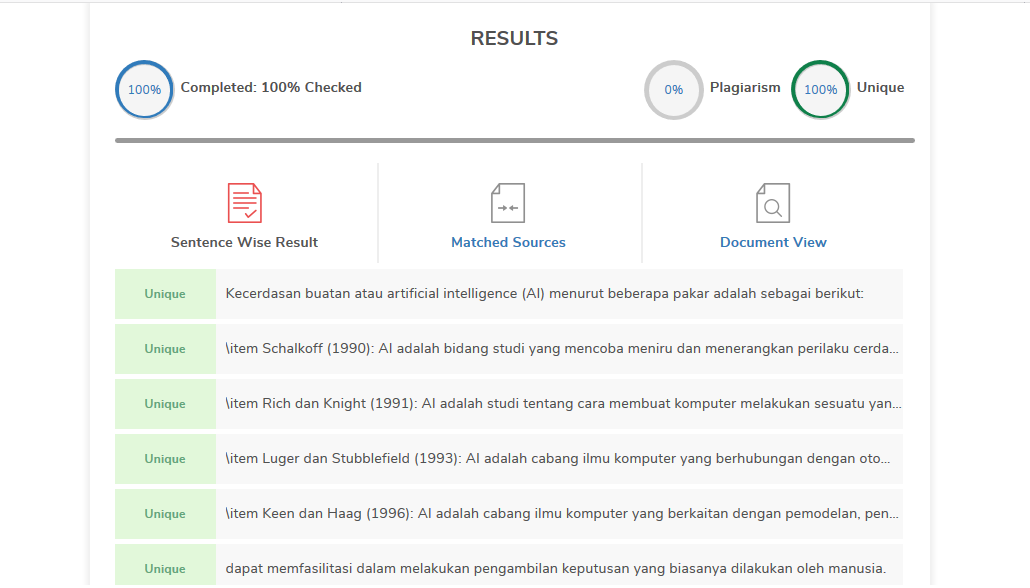
\includegraphics[width=1\textwidth]{figures/1174006/chapter1/plagiat.png}
	\centering
	\caption{Bukti Tidak Plagiat.}
\end{figure}